\documentclass[12pt, twoside]{article}
\usepackage[letterpaper, margin=1in, headsep=0.5in]{geometry}
\usepackage[english]{babel}
\usepackage[utf8]{inputenc}
\usepackage{amsmath}
\usepackage{amsfonts}
\usepackage{amssymb}
\usepackage{tikz}
\usetikzlibrary{quotes, angles}
\usepackage{graphicx}
\usepackage{enumitem}
\usepackage{multicol}

\newif\ifmeta
\metatrue %print standards and topics tags

\title{Regents Geometry}
\author{Chris Huson}
\date{November 2021}

\usepackage{fancyhdr}
\pagestyle{fancy}
\fancyhf{}
\renewcommand{\headrulewidth}{0pt} % disable the underline of the header
\raggedbottom


\fancyhead[LE]{\thepage}
\fancyhead[RO]{\thepage \\ Name: \hspace{4cm} \,\\}
\fancyhead[LO]{BECA / Dr. Huson / Geometry 04 Analytic Geometry}

\begin{document}

\subsubsection*{4.13 Classwork: Density}
\begin{enumerate}
  \item Find the area of the shape shown below composed of a rectangle and a semi-circle.
  \begin{flushright}
  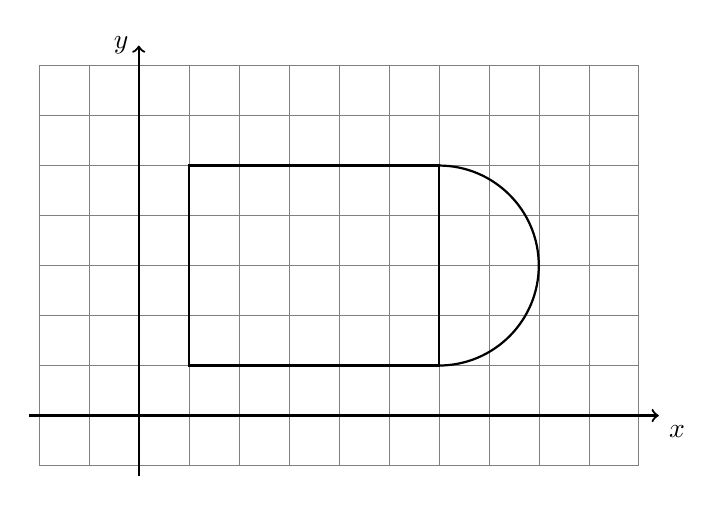
\begin{tikzpicture}[scale=.635]
    \draw [help lines] (-2,-1) grid (10,7);
    \draw [thick, ->] (-2.2,0) -- (10.4,0) node [below right] {$x$};
    \draw [thick, ->] (0,-1.2)--(0,7.4) node [left] {$y$};
    \draw [thick] (1,1)--(6,1)--(6,5)--(1,5)--cycle;
    \draw [thick] (6,1) arc (-90:90:2);
  \end{tikzpicture}
\end{flushright}

\item A cylinder is 12.3 cm tall and has a volume of 966 cubic cm. Find the area of the base of the cylinder. Express your result to the \emph{nearest hundredth of a square centimeter}. \vspace{3cm}

\subsubsection*{Applying density ratios}
\item Find the weight of a metal block with a volume of 20 cubic inches and a density of 0.75 pounds per cubic inch. \vspace{3cm}
\item A large block of ice has a volume of 45 liters. The density of ice (water) is one kilogram per liter. Find the weight of the ice.  \vspace{3cm}
\item A tank of gasoline holds 20 gallons. Find the cost to completely fill the tank if gasoline costs \$2.35 per gallon. \vspace{3cm}
\item A bar of solid gold is in the shape of a rectangular prism having a length of 10 cm, width of 4 cm, and thickness of 1.5 cm. The density of gold is 19.3 grams per cubic cm, and its approximate market value is \$50 per gram.
\begin{enumerate}
  \item Find the weight of the bar of gold.  \vspace{3cm}
  \item Find its value in dollars.\vspace{2cm}
\end{enumerate}


\subsubsection*{Model the situation with an equation. \hfill Do NOT solve!}

  \item A large concrete post in the shape of a cylinder has a volume of 250 cubic feet. Its height is 12 feet. Find the radius of the base of the post. \vspace{2cm}

  \item A spherical cork fishing net float has a volume of 4000 cubic centimeters. Find its radius. \vspace{2cm}

  \item The volume of a cone having a \textbf{diameter} of 10 inches is 200 cubic inches. Find the cone's height.


\end{enumerate}
\end{document}